
\documentclass[english]{beamer}
\usepackage{mathpazo}
\usepackage[T1]{fontenc}
\usepackage[latin9]{luainputenc}
\setcounter{secnumdepth}{3}
\setcounter{tocdepth}{3}
\setlength{\parskip}{\smallskipamount}
\setlength{\parindent}{0pt}
\usepackage{amsthm}
\usepackage{amssymb}
\usepackage{graphicx}
\usepackage{setspace}
\onehalfspacing

\makeatletter
\providecommand{\tabularnewline}{\\}

%%%%%%%%%%%%%%%%%%%%%%%%%%%%%% Textclass specific LaTeX commands.
% this default might be overridden by plain title style
\newcommand\makebeamertitle{\frame{\maketitle}}%
% (ERT) argument for the TOC
\AtBeginDocument{%
  \let\origtableofcontents=\tableofcontents
  \def\tableofcontents{\@ifnextchar[{\origtableofcontents}{\gobbletableofcontents}}
  \def\gobbletableofcontents#1{\origtableofcontents}
}
\numberwithin{equation}{section}
\numberwithin{figure}{section}
\theoremstyle{plain}
\newtheorem{thm}{\protect\theoremname}
\theoremstyle{definition}
\newtheorem{defn}[thm]{\protect\definitionname}

%%%%%%%%%%%%%%%%%%%%%%%%%%%%%% User specified LaTeX commands.
\usetheme[progressbar=frametitle]{metropolis}
\usepackage{appendixnumberbeamer}

%\usepackage{booktabs}
%\usepackage[scale=2]{ccicons}

%\usepackage{pgfplots}
%\usepgfplotslibrary{dateplot}

%\usepackage{xspace}
%\newcommand{\themename}{\textbf{\textsc{metropolis}}\xspace}

\makeatother

\usepackage{babel}
\providecommand{\definitionname}{Definition}
\providecommand{\theoremname}{Theorem}

\begin{document}
\title{Rotations and the Spin $1/2$ Particle in a Magnetic Field}
\author{Emmanuel Flores}
\date{\today}
\institute{Advanced Mathematical Methods, Tufts University}

\makebeamertitle

\section*{Spinor Representation}
\begin{frame}{Some Motivation}

\begin{itemize}
\item The existence of spin $1/2$ particles shows that is $Spin\left(3\right)$
rather than $SO\left(3\right)$ that is the symmetry group of corresponding
of rotations of fundamental quantum systems.
\item The idea is to study $\mathcal{H}=\mathbb{C}^{2}$ with the group
action given by rotations in $3D$.
\end{itemize}
\begin{defn}
The spinor representation of $Spin\left(3\right)=SU\left(2\right)$
is the representation on $\mathbb{C}^{2}$ given by 
\[
g\in SU\left(2\right)\rightarrow\pi_{spinor}\left(g\right)=g,
\]
and elements of the representation space $\mathbb{C}^{2}$ are called
spinors.
\end{defn}

\end{frame}

\section*{Spin $\frac{1}{2}$ in a Magnetic Field}
\begin{frame}{Elements of the Lie algebra}
\begin{itemize}
\item We will consider only the $SU\left(2\right)$ subgroup of $U\left(2\right)$.
\item ``When it occurs in its role as double cover of the rotational group,
the quantum system is said to carry \textquotedblleft spin\textquotedblright ,
in particular \textquotedblleft spin $1/2$\textquotedblright{} for
the two dimensional irreducible representation.''
\item Elements of the Lie algebra 
\[
X_{j}=-i\frac{\sigma_{j}}{2},
\]
with commutation relations 
\[
\left[X_{1},X_{2}\right]=X_{3},\hspace{1em}\left[X_{2},X_{3}\right]=X_{1},\left[X_{3},X_{1}\right]=X_{2}.
\]
\end{itemize}
\end{frame}
%
\begin{frame}{Physics Connection}
\begin{itemize}
\item Making contact with physics 
\[
S_{j}=i\hbar X_{j},
\]
we like this as observables because the eigenvalues are real $\pm1/2$
(experimental measures).
\item Elements of the group are given by 
\[
\Omega\left(\theta,\mathbf{w}\right)=\exp\left(-\frac{i}{\hbar}\mathbf{w}\cdot\mathbf{S}\right)\in SU\left(2\right).
\]
\item States in $\mathcal{H}$ that have a well-defined value of the observable
$S_{j}$ will be eigenvectors of $S_{j}$ with eigenvalues $\pm1/2.$
\end{itemize}
\end{frame}
%
\begin{frame}{Action of $\Omega$ }
\begin{itemize}
\item Let $\left|\psi\right\rangle \in\mathcal{H}$, thus we have 
\[
\left|\psi\right\rangle \rightarrow\Omega\left|\psi\right\rangle .
\]
\item Baker-Hausdorff lemma 
\begin{align*}
\exp\left(iG\lambda\right)A\exp\left(-iG\lambda\right) & =A+i\lambda\left[G,A\right]\\
 & +\left(\frac{i^{2}\lambda^{2}}{2!}\right)\left[G,\left[G,A\right]\right]+\dots
\end{align*}
\end{itemize}
\end{frame}
%
\begin{frame}{The Hamiltonian}
\begin{itemize}
\item The spin degree of freedom that we are describing by $\mathcal{H}$
has a dynamics given by 
\[
\mathbf{H}=-\mu\cdot\mathbf{B},
\]
where 
\[
\mu=-\frac{ge}{2mc}\mathbf{S},
\]
is the magnetic moment operator.
\end{itemize}
\end{frame}
%
\begin{frame}{With Schr�dinger Equation}

The Schr�dinger equation is given by
\[
\frac{d}{dt}\left|\psi\right\rangle =-i\left(-\mu\cdot B\right)\left|\psi\right\rangle 
\]
and solution 
\[
\left|\psi\left(t\right)\right\rangle =U\left(t\right)\left|\psi\left(0\right)\right\rangle ,
\]
where 
\[
U\left(t\right)=\exp\left(it\mu\cdot B\right).
\]

\end{frame}
%
\begin{frame}{Explicitly}
\begin{itemize}
\item Assuming $\mathbf{B}$ with just a component in the $z$-direction,
we have
\[
\mathbf{H}=\omega S_{z},
\]
thus 
\[
U\left(t\right)=\exp\left(-\frac{iS_{z}\omega t}{\hbar}\right),
\]
we see that this Hamiltonian causes spin precession.
\end{itemize}
\begin{minipage}[t]{1\columnwidth}%
\begin{center}
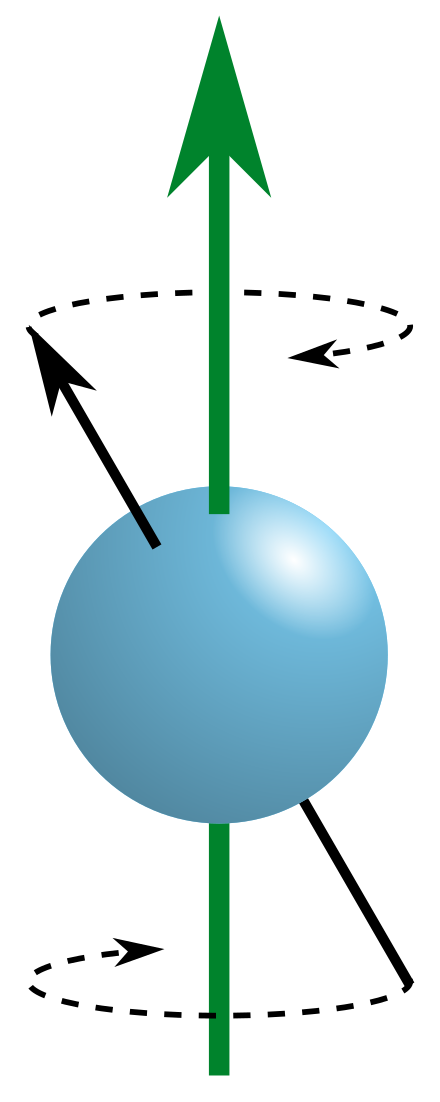
\includegraphics[scale=0.1]{Precession_in_magnetic_field}
\par\end{center}%
\end{minipage}
\end{frame}
%
\begin{frame}{Physical Systems}
\begin{itemize}
\item The Zeeman effect,
\item Stern Gerlach experiment,
\item Nuclear magnetic resonance spectroscopy,
\item Quantum computing.
\end{itemize}
\end{frame}

\section*{Heisenberg Picture}
\begin{frame}{Schr�dinger and Heisenberg Pictures}

\begin{minipage}[t]{1\columnwidth}%
\begin{center}
\begin{tabular}{|c|c|c|}
\hline 
 & Heisenberg Picture & Schr�dinger Picture\tabularnewline
\hline 
\hline 
State Ket & No Change & Evolution Given by $H$\tabularnewline
\hline 
Observable & Evolution Given by $H$ & No Change\tabularnewline
\hline 
\end{tabular}
\par\end{center}%
\end{minipage}

\end{frame}

\section*{Complex Projective Space}
\begin{frame}{Trying Another Characterization}
\begin{itemize}
\item Multiplication on $\mathcal{H}$ by non-zero complex number do not
change eigenvectors $\implies$ no physical effect.
\item The relevant part is the quotient space $\left(\mathbb{C}^{2}-\left\{ 0\right\} \right)/\mathbb{C}^{*}$,
and constructed by: taking all non-zero elements of $\mathbf{C}^{2}$
and identifying those related by multiplication by a non-zero complex
number.
\item In some sense the space $CP^{1}$ is the complex plane, but with a
\textquotedblleft point at infinity\textquotedblright{} added.
\end{itemize}
\end{frame}
%
\begin{frame}{Riemann Sphere}
\begin{itemize}
\item $CP^{1}$: \textquotedblleft Riemann sphere\textquotedblright{} with
the relation to the plane and the point at infinity given by stereographic
projection.
\end{itemize}
\begin{minipage}[t]{1\columnwidth}%
\begin{center}
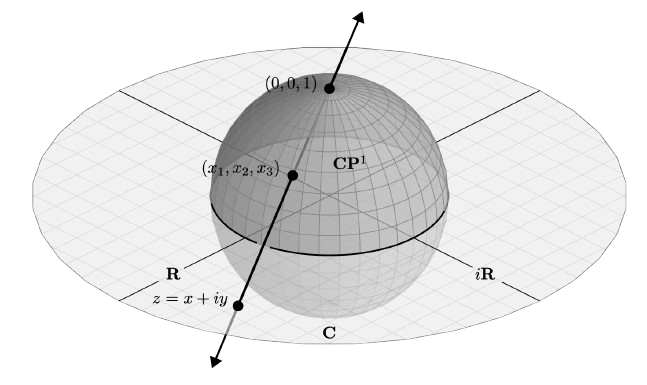
\includegraphics[scale=0.25]{Stereo_Projection}
\par\end{center}%
\end{minipage}

\end{frame}
%
\begin{frame}{Coordinates relationship}

\begin{itemize}
\item Relation between coordinates on the sphere $\left(x_{1},x_{2},x_{3}\right)$
and complex coordinates $z_{1}/z_{2}=z=x+iy$ is given by 
\[
x=\frac{x_{1}}{1-x_{3}},y=\frac{x_{2}}{1-x_{3}},
\]
and 
\[
x_{1}=\frac{2x}{x^{2}+y^{2}+1},x_{2}=\frac{2y}{x^{2}+y^{2}+1},x_{3}=\frac{x^{2}+y^{2}-1}{x^{2}+y^{2}+1}
\]
\end{itemize}
\end{frame}

\section*{The Bloch Sphere}
\begin{frame}{Another Characterization}
\begin{itemize}
\item The unit sphere $S^{2}\subset\mathbb{R}^{3}$ can be mapped to operators
by 
\[
\mathbf{x}\rightarrow\sigma\cdot\mathbf{x},
\]
and for each point $\mathbf{x}\in S^{2}$, $\sigma\cdot\mathbf{x}$
has eigenvalues $\pm1$. Eigenvectors with eigenvalue $+1$ are solutions
to 
\[
\sigma\cdot\mathbf{x}\left|\psi\right\rangle =\left|\psi\right\rangle .
\]
\end{itemize}
\end{frame}
%
\begin{frame}{Interpretation in terms of spin operators}

\begin{itemize}
\item One can characterize the $\mathbb{C}\subset\mathcal{H}$ corresponding
to $\mathbf{x}\in S^{2}$ as the solutions to 
\[
\mathbf{S}\cdot\mathbf{x}\left|\psi\right\rangle =\frac{1}{2}\left|\psi\right\rangle ,
\]
thus, the North pole of the sphere is a ``spin-up'' state and the
South pole is a ``spin down'' state.
\item Along the equator one finds two points corresponding to states with
definite values for $S_{1}$, as well as two for states that have
definite values for $S_{2}$.
\end{itemize}
\end{frame}

\end{document}
